\chapter{23 Gennaio 2017 - Biliardi ellittici e Funzioni Modulari}
\justify

\section{Biliardi ellittici}
\newthought{Introduciamo un altro modo} in cui si ottengono le curve
ellittiche dalle ellissi \notamargine{Abbiamo infatti già visto che si
  possono ottenere come integrali della lunghezza d'arco di un'ellisse}.

Prendiamo un'ellisse di equazione $ax^2 + by^2 = 1$ e supponiamo di
giocare a biliardo sull'ellisse: facendo partire la pallina da un punto
la lanciamo contro il bordo dell'ellisse su cui rimbalza secondo la nota
legge \notamargine{Ovvero rispetto alla tangente all'ellisse nel punto
  rimbalza via con lo stesso angolo, come indicato in figura}

\begin{center}
  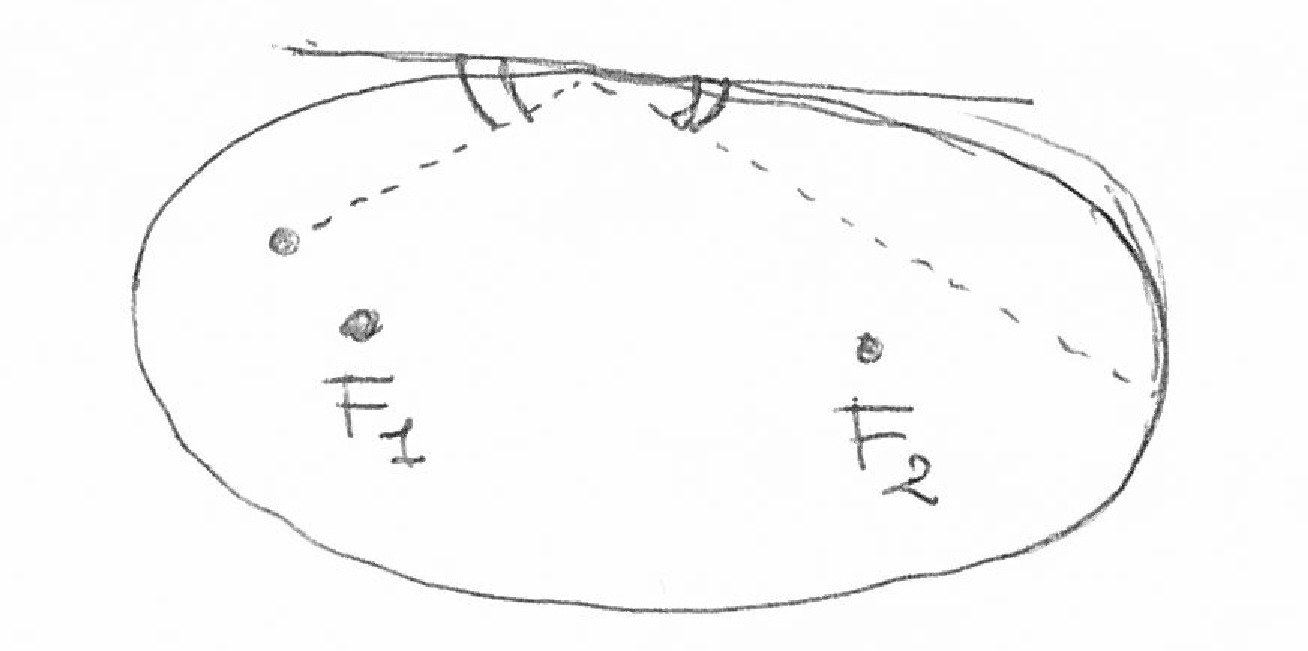
\includegraphics[width=3cm]{lezione-170123-fig1}
\end{center}
  
Una cosa che è nota da tempo è che le rette che compongono la
traiettoria sono tutte tangenti ad un'altra ellisse ``caustica'' che ha
gli stessi fuochi della prima: abbiamo quindi una famiglia ad un
parametro di ellissi che descrive tutte le possibili traiettorie.

\newthought{Vediamo allora che succede} quando prendiamo un punto $P$
sul bordo dell'ellisse ed una retta $l$ con $P \in l$ e tangente alla
caustica.

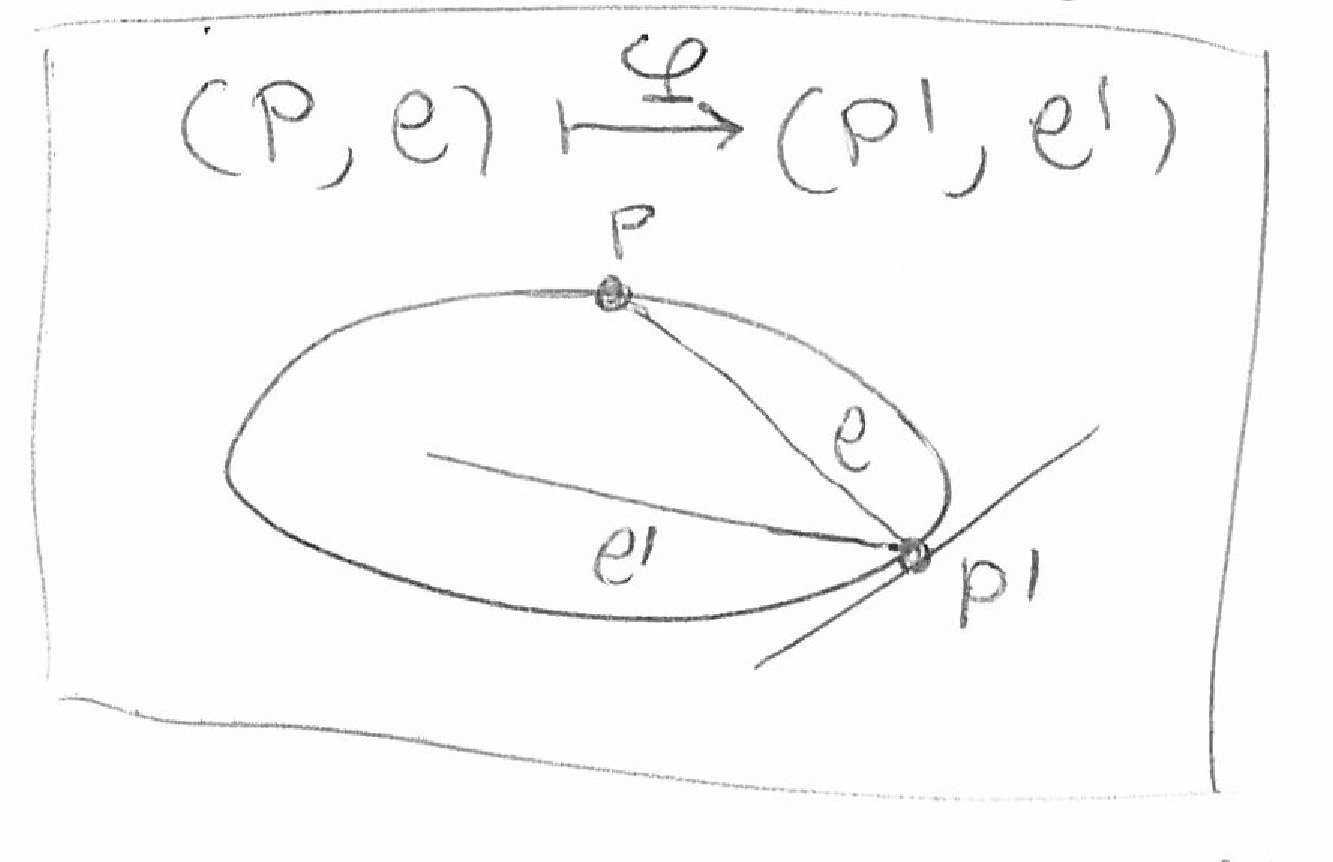
\includegraphics[width=3cm]{lezione-170123-fig2}
% TODO: Finire paragrafo che diventa bruttissimo

\section{Funzioni Modulari}

\notamargine{Il nome ``modulari'' è riferito ai moduli, parametri che
  comparivano negli integrali ellittici. Oggi ci si riferisce a moduli
  per indicare uno spazio di parametri per una famiglia di curve
  algebriche.

  Esempio ``stupido'': $y - a x^2 = 0$ al variare di $a \in \bbC$ sono
  una famiglia di parabole (o per $a=0$ una retta). In questo caso lo
  spazio dei parametri è $\bbC$ (nel quale $a$ può variare)}

\begin{osservazione}
  Ricordiamo che conosciamo già un parametro delle cubiche:
  $j$. Infatti, se la cubica viene da un toro allora è della forma
  $y^2 = 4 x^3 - g_2 x - g_3$ e sappiamo che
  $j = 1728 \frac{g_2^3}{g_2^3 - 27 g_3^2}$ è un'invariante per
  trasformazioni algebriche delle cubiche.
\end{osservazione}

Siamo allora autorizzati a riscalare il reticolo $L$ pur restando nella
stessa classe di isomorfismo delle cubiche. Possiamo quindi supporre che
$L = \bbZ \tau + \bbZ 1$ con $\tau \in \cH = \{ z \in \bbC | \Img \tau >
0 \}$. In questo modo $g_2 = 60 \sum_{\omega \in L^*} \omega^{-4}$ e
$g_3 = 140 \sum_{\omega \in L^*} \omega^{-6}$ diventano funzioni
olomorfe di $\tau$ come parametro nel semipiano superiore e quindi pure
$j$ è una funzione di $\tau$

\begin{osservazione}
  Se vedessimo che $j$ assume tutti i valori in $\bbC$ ciò dimostrerebbe
  che tutte le cubiche provengono da un toro, poiché sappiamo già che
  due cubiche sono affinemente equivalenti se e solo se hanno lo stesso $j$.
\end{osservazione}

\begin{divagazione}
  Si può dimostrare che $\tau$ è immaginario quadratico su $\bbQ$ allora
  $j(\tau)$ è un numero algebrico. Di seguito diamo un'idea della dimostrazione
  \notamargine{ Immaginario quadratico vuol dire che soddisfa
    un'equazione di secondo grado a coefficienti in $\bbQ$, ovvero $x$ è
    tale che $\exists b, c \in \bbQ$ con $x^2 + bx + c = 0$}

  Quando $\tau$ è un immaginario quadratico il reticolo ha infatti degli
  automorfismi non banali. Se $j$ fosse trascendente, visto che gli
  automorfismi sono funzioni razionali delle coordinate e avremmo
  $\bbQ(j, funz.raz.)$ come campo finitamente generato su $\bbQ$, che ha
  però grado di trascendenza uno.

  Allora si può specializzare $j$, visto che il campo è isomorfo ad una
  cosa con una variabile. Specializzandolo ad ogni altro numero
  trascendente ottengo un campo isomorfo e quindi tutte le curve
  ellittiche avrebbero degli automorfismi non banali (poiché hanno
  uguali campi) e ciò è impossibile poiché le cubiche con automorfismi
  sono in numero numerabile.
\end{divagazione}

\section{Costruzione di un dominio fondamentale}

\begin{center}
  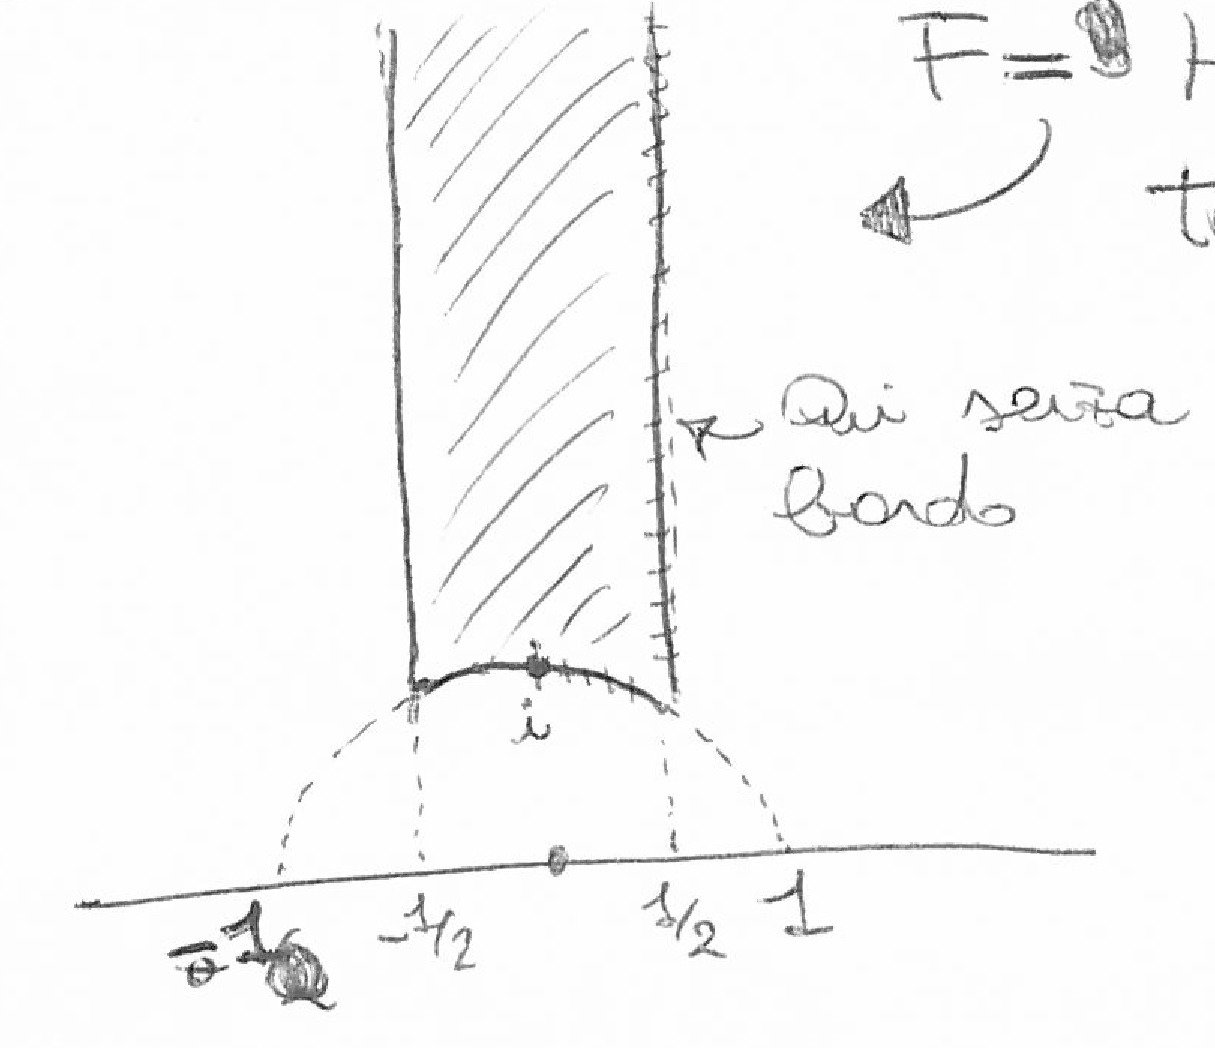
\includegraphics[width=8cm]{lezione-170123-fig3}
\end{center}

